%!TEX root = ../../dissertation.tex
%%%%%%%%%%%%%%%%%%%%%%%%%%%%%%%%%%%%%%%%%%%%%%%%%%%%%%%%%%%%%%%%%%%%%%%%%%%%%%%%
%%%%%%%%%%%%%%%%%%%%%%%%%%%%%%%%%%%%%%%%%%%%%%%%%%%%%%%%%%%%%%%%%%%%%%%%%%%%%%%%
%%%%%%%%%%%%%%%%%%%%%%%%%%%%%%%%%%%%%%%%%%%%%%%%%%%%%%%%%%%%%%%%%%%%%%%%%%%%%%%%
\section{Streaming Modeling}
\label{c3:sec:modeling}

As web-based delivery uses reliable TCP transfers and (in its simplest form) does not use any kind of scaling or multi-layered video encoding, there will never be any change in the actual video quality. Therefore, the users' experience is influenced by only a small number of parameters. A user will notice some delay after he starts the video streaming process. If the video download is slower than the average video bitrate the playback will stall, i.e. stop playing, at some point until there is enough data available to resume playing again.
The QoS parameters affecting these metrics are limited bandwidth, packet loss, and latency, causing the player to intermittently pause playback and enter a re-buffering state.

Directly measuring these two factors in a user-controlled browser does have drawbacks. The need for user interaction would hamper the effort of creating fully automated measurement series and getting reproducible results. Interfacing with the closed-source Flash software and getting meaningful results can also be a large hurdle.

To achieve increased flexibility we created several models that emulate the streaming process and its buffering and playback behavior. These are based on typical user playback solutions, e.g. a Web browser with a Flash plug-in. For this comparison we used a video of about 90 seconds length and network conditions that could not fulfill the video bitrate in time and hereby forced stalling to occur.

While these models try to give dimensions and characteristics to the initial start delay and the frequency and lengths of stalls they do not directly answer the question of user satisfaction. Approaches to correlate the  measurable parameters and the user satisfaction are tackled in, e.g., \cite{ketyko2010qoe, mokmeasuring, gustafsson2008measuring} and will also be a topic of our future work.


\begin{figure}[htbp]
%\vskip -2.5cm
        \centering
        % \begin{subfigure}[b]{0.50\textwidth}
        %         \centering
        %         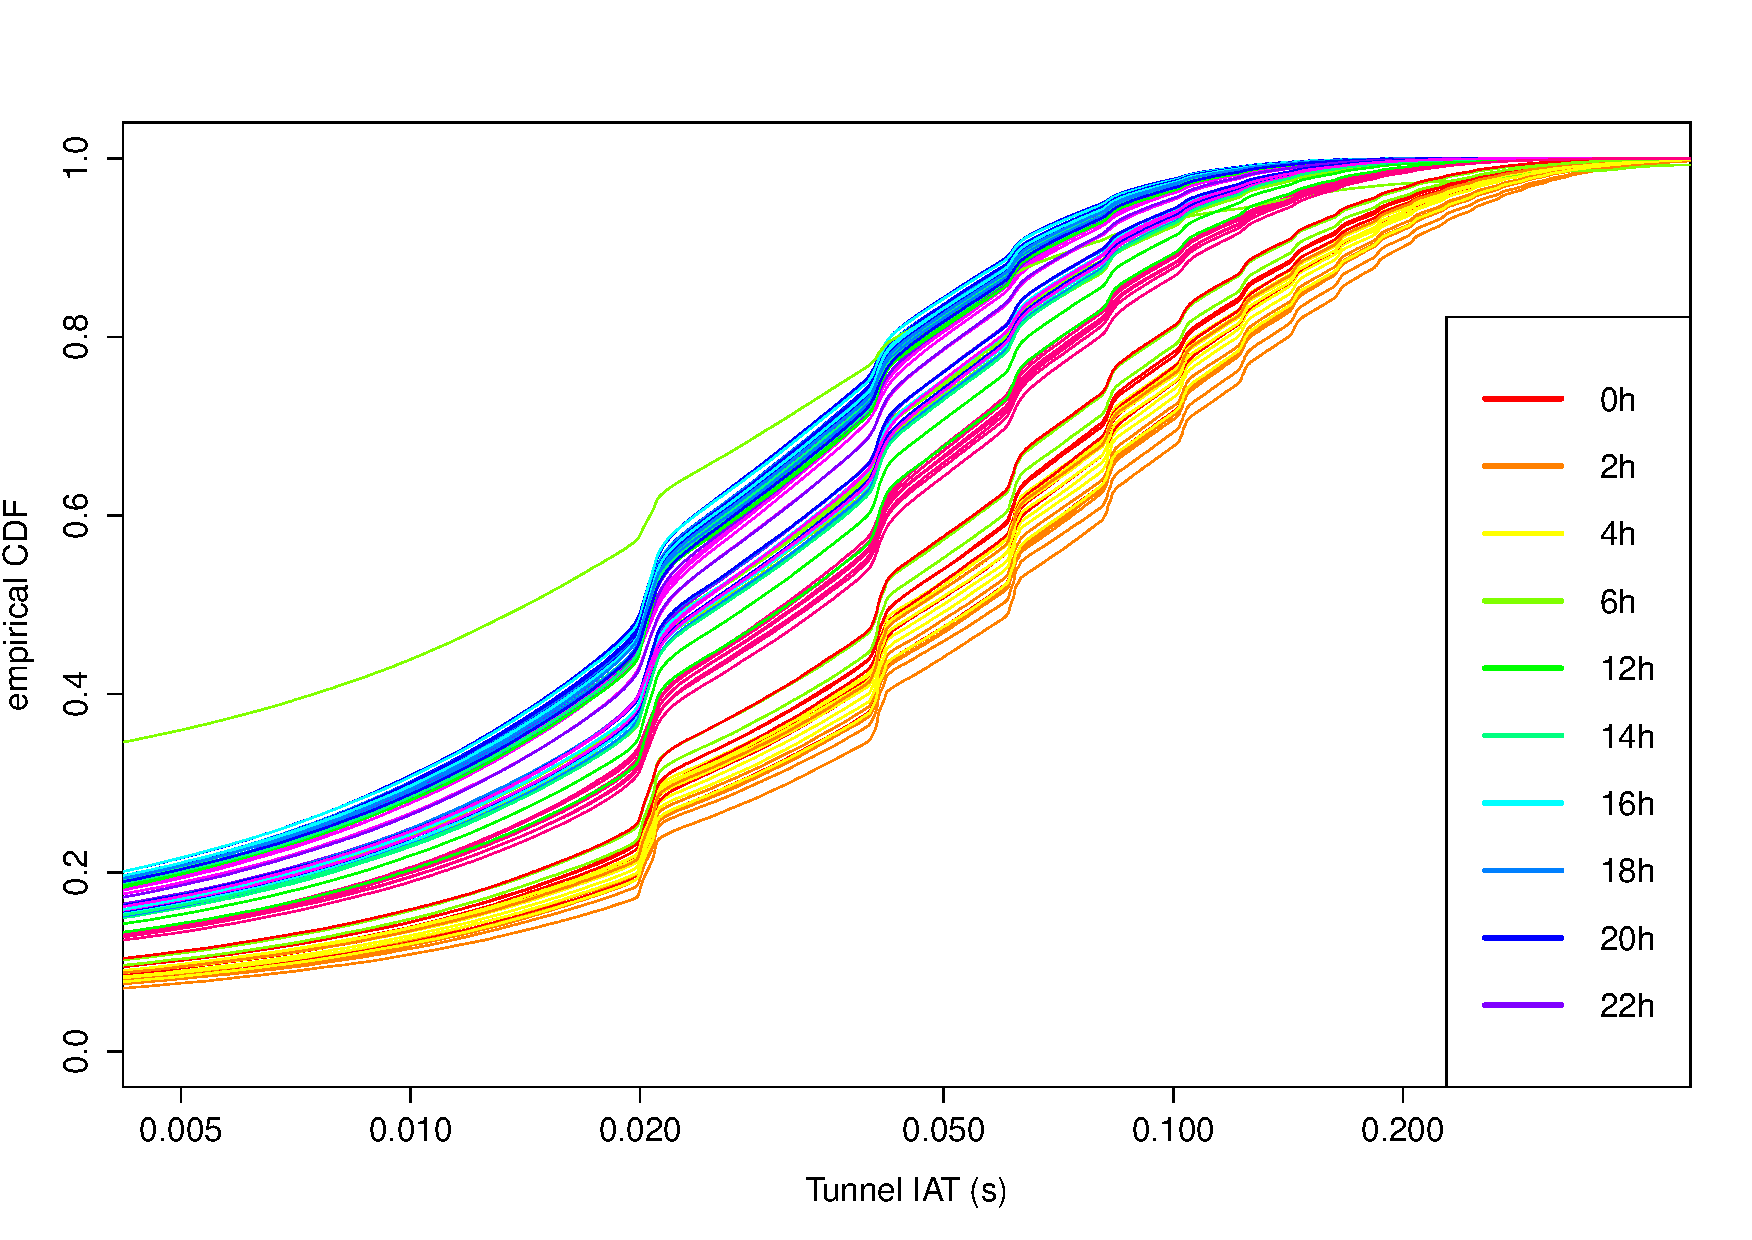
\includegraphics[width=\textwidth]{figures/R-IAT-ecdf-2h-log.png}
        %         \caption{All incoming tunnel requests.}
        %         \label{fig:IAT-ecdf-2h-all}
        % \end{subfigure}%
        %~ %add desired spacing between images, e. g. ~, \quad, \qquad etc.
          %(or a blank line to force the subfigure onto a new line)
        \begin{subfigure}[b]{0.50\textwidth}
                \centering
                \includegraphics[width=\textwidth]{images/bufferlevel-stall-new.pdf}
                \caption{Playback stalling method, 33s total stalling.}
                \label{c3:fig:bufferlevel-stall}
        \end{subfigure}%
        ~
        \begin{subfigure}[b]{0.50\textwidth}
                \centering
                \includegraphics[width=\textwidth]{images/bufferlevel-startdelay-new.pdf}
                \caption{Delayed playback method, 33s total stalling.}
                \label{c3:fig:bufferlevel-startdelay}
        \end{subfigure}

        \begin{subfigure}[b]{0.50\textwidth}
                \centering
                \includegraphics[width=\textwidth]{images/bufferlevel-flash-new.pdf}
                \caption{YouTube Flash Player method, 34s total stalling.}
                \label{c3:fig:bufferlevel-flash}
        \end{subfigure}%
        ~
        \begin{subfigure}[b]{0.50\textwidth}
                \centering
                \includegraphics[width=\textwidth]{images/bufferlevel-firefox-new.pdf}
                \caption{Firefox 4 method, 44s total stalling.}
                \label{c3:fig:bufferlevel-firefox}
        \end{subfigure}
\caption{Modelled buffer fill level graphs and resulting total stalling times.}
\label{c3:fig:bufferlevel-PV}
\end{figure}
% used yt-delay/hPUGNCIozp0_delay_2500 1, spyder, color #aa5500
% data
% start delay 33s 
% flash 33.82s
% stalling 32.68s
% html5 as implemented in firefox 44s

\subsection{Simple Stalling Model}

The simplest version of the model is represented in Figure \ref{c3:fig:bufferlevel-stall} which shows the difference between the aggregate downloaded and already played data, which is the buffer level. The model starts and advances playback immediately when it has enough data to show a full frame and stops every time the buffer is about to run out and restarts immediately when there is data to show. This results in numerous stops and a large loss in playback continuity. However, this model also has the shortest total stalling time and can therefore act as a reference baseline to compare the performance of the other models against it.


\subsection{Simple Predictive Model}

The second approach in Fig. \ref{c3:fig:bufferlevel-startdelay} defers the playback start as long as it is needed to play the video uninterrupted, meaning that the playback buffer will never run out of data. However, this approach is only viable with a complete knowledge over the downloading process, which can only be estimated in live scenarios. Because playback is done with global knowledge and at the earliest point possible the total stalling time is also 33 seconds, but only one long stalling phase occurs while the user initially waits for the playback to start.


\subsection{YouTube Model}

This model tries to resemble the playback mechanisms as implemented in YouTube's Flash video player.
It defers the start until at least two seconds of video data are buffered. When a stall occurs the player buffers at least five seconds of video before restarting. The model does not use any knowledge about the transmission (e.g. current bandwidth).
The result can be seen in Figure \ref{c3:fig:bufferlevel-flash}. Compared to the simple stalling model it increases the playback stability while only marginally affecting the total stalling time, resulting in 34 seconds of stalling.

\subsection{HTML5 Predictive Model}
The standard playback and buffering process of HTML5 is described in the HTML5 specification but adds up to:
\textit{``[...] the user agent [...] will automatically begin playback of the media resource as soon as it can do so without stopping.''} \cite{html5video}. The model presented here is based on the HTML5 implementation of the open source Firefox Browser in version 4 which differs slightly from the HTML standard. Because it is an online algorithm which does not have global knowledge of the video and transmission speeds of any point in the future it has to estimate these. It does so by calculating the moving averages of both. Playback is started when one of these conditions are met:

\begin{itemize}
\item The player has been buffering data for at least 30 seconds.
\item The player has already buffered an amount of data corresponding to 30 seconds of video.
\item The video download has been completed.
\item The moving average of the transmission rate is larger than the moving average of the video bitrate and the player has a safety buffer with 20 seconds of video data.
\end{itemize}

This approach is quite conservative and trades longer waiting times for fewer interruptions. The test case for our model is shown in Figure \ref{c3:fig:bufferlevel-firefox}. Initially, playback starts only after a long waiting period of about 25 seconds. Also, the only intermittent stall causes a long buffering period. Then again, the model keeps the total number of stalls down to this single stall. However, due to the longer overall stalling time of 44 seconds the player needs to buffer more data than the other model implementations. In our test case the maximum buffer size increased from about 2800 KiB to 5600 KiB. This may be a problem for devices with sparse amounts of memory, e.g. mobile telephones or small dedicated streaming boxes. However, a large buffer can also increase the chance of continuous playback in mobile scenarios with intermittent service interruption.


%Which offers better quality to users? Some approaches (TODO: refs and explain how)

% Longer waiting time but very few stops. Stalling model definitely the shortest waiting time but stops too frequent with insufficient network conditions, i.e. can not really be used. Delayed playback requires total knowledge not available beforehand. Can maybe used with reduced information, bandwidth estimation, but this is essentially HTML5/Firefox.



\subsection{Application Behavior}

The time scale on which streaming applications buffer content lies in the range of seconds. This is a necessity in a best-effort network, as the available network bitrate might drop unexpectedly and could drain a shallower buffer quickly. % On the other hand, given sufficient band-width or even bandwidth guarantees as demanded in SAE, buffer sizes could be reduced, improving interactivity of the stream and enabling closer-to-realtime live streaming or conferencing.
The application behavior represents a trade-off between different types of perceivable artifacts -- initial startup delay, stalls, (partial) media skips (e.g. continuous audio, but skipping video), and quality adaption. The next Section will specifically look at these issues.




%%%%%%%%%%%%%%%%%%%%%%%%%%%%%%%%%%%%%%%%%%%%%%%%%%%%%%%%%%%%%%%%%%%%%%%%%%%%%%%%
\subsection{Application Behavior}

%This section provides an analysis of different playback models, both hypothetical best/worst-case, and actually implemented ones. We set off to develop a generic model for the playback process of a streaming application, and then explore the result space yielded by the application behavior.
%
%\subsection{Generic playback model}

To play back a media stream, an application needs to maintain a media buffer of sufficient size to at least gather enough data to reconstruct one single atomic unit of playback such as a video frame.

The current buffer level at time $t$ is given by the amount of data received from the network so far, diminished by the amount of data already played back. The actual media format used in the stream determines the progress of the playback process, whereas the network conditions and application download strategies yield the overall progress of data reception:

\begin{equation*}
\mathit{buffer}(t) = \sum_{0}^{t} data_\mathrm{received} - \sum_{0}^{t} data_\mathrm{played}
\end{equation*}
 
The playback buffer level governs how well the player can conduct the playback. If the buffer reaches zero size the playback process stops and stalling occurs. Then a decision is required when to restart the playback process again after a stall, and if the stream should skip forward to a more current playback position. This process is the core part of the playback model for an HTTP streaming service. The model could also be extended to accommodate adaptive streaming mechanisms that feed back the buffer level to influence the download strategy of the player, e.g. send a receiver report to request a lower-bitrate stream in the case of RTP. % Consequently, the progress of data received would increase at a lower rate, and the playback rate would decrease as well once the residual stream data in the buffer were played out.

Playback models need to define the behavior at the occurrence of one of two conditions during the playback process. These are the initial playout delay (the point in time when to start draining the playback buffer), and the buffer fill level at which to start playing again if the buffer had intermittently emptied and the video had to be stopped.

These decisions yield a stalling period distribution for a streamed video. The frequency and the duration of stalls directly relate to the decision function of the playback model. The more frequent the stalls are, the shorter they will be; if the function produces longer stalls, they will be less frequent.

There can be other parameter spaces governed in the model. For example, in a live streaming scenario a user could prefer to always stay at the most current stream position. To enable this, a player would skip older parts of the video. If the user prefers to consume the entire stream, the player would show the video without skipping parts, but pause intermittently. 

Another user parameter is the quality level of the video for adaptive streaming. This trades off between maintaining a certain quality level and putting up with increased waiting times, and dropping the quality to a level sustainable at the current transmission rate.

%\begin{figure}[!t] % use 1.75in each for single-column
%\centering
%\includegraphics[width=0.8\textwidth]{usersatisfaction}
%\caption{User Experience as a trade-off between stalls and start-up delay}
%\label{fig:stalltradeoff}
%\end{figure}

% As sketched for the start-up delay and the number of stalls in Figure \ref{fig:stalltradeoff}, all of these resulting parameter spaces could in turn be mapped to user satisfaction metrics describing the user's experienced quality. 
% However, this mapping goes beyond the scope of this work. The focus is rather on the creation of simple evaluation methods to assign combinations of network conditions and playback models to specific stalling characteristics defining a base for user satisfaction decisions.

The next subsections present four stalling playback models, ranging from theoretical models that represent boundaries to the values possible in stalling characteristics, to the Firefox and the Flash model, which represent actual player behaviors that can be seen ``in the wild''.


\subsection{Simple Playback Stalling Model}
The behavior can be summarized as ``Whenever anything can be played from the buffer, do so''. This means that, if the player is currently stalling and a complete frame becomes available in the buffer, playback will immediately restart and the frame will be shown even if this means stopping playback after that frame again. This results in the lowest required buffer space. Moreover, it gives an upper limit for the number of stalls occurring\footnote{As a video frame is atomic, no other model could possibly stop the playback more often.}.

\subsection{Initial Playback Delay Model}
The model is similar to progressively downloading the whole stream, as it will simply delay the initial start of the video until it can be played completely without any buffer underruns occurring. The only stall occurring is the initial waiting period until the video starts. The time spent waiting will also be minimal. The downside of this model is its use of perfect knowledge on the future network conditions at any point in time, making it purely theoretical. Actual streaming players need to accurately predict the transmission process, e.g. through moving averages.


The stalling and initial delay models define the maximum achievable upper and lower limits for the stalling parameter space for all possible real models.


\subsection{Firefox HTML5 Model}
The algorithm used in the Firefox 4 browser is an approximate realization of the HTML5 video standard \cite{html5} which suggests starting the playback only when it can be ensured that the video can be played without interruption similar to the initial playback delay model.

The algorithm and its variables are shown in Algorithm \ref{c3:alg:firefox-PV} and Table \ref{c3:tbl:buffvars}, respectively. Firefox 4 uses moving averages to estimate the development of the transmission rate. It does not differentiate between intermittent and initial conditions. As the approach is similar in concept to the initial playback delay model, %it results in a very large required buffer space, but also %
it sports very few stalling events due to conservatively chosen (i.e., long) buffering times.



\begin{figure}[htbp]
    \centering
    \begin{algorithmic}
        \IF {$s_{MA} > v_{MA}$} 
          \STATE $c \gets ( b_b=20s \lor b_T=20s )$
        \ELSE
          \STATE $c \gets ( b_b=30s \lor b_T=30s )$
        \ENDIF 
    \end{algorithmic}
    \caption{Firefox playback (re-)start decision algorithm.}
    \label{c3:alg:firefox-PV}
\end{figure}


\begin{table}[htbp]
    \caption{Variables involved in buffering decisions.}
    \label{c3:tbl:buffvars}
    \centering
    \begin{tabu}{|l|X[p]|} 
    \hline
    Variable & Description \\ \hline
    $s_{MA}$ & Moving average of the transmission speed. \\
    $v_{MA}$ & Moving average of the video bitrate. \\ 
    $c$   & Condition upon which to start/resume playback. \\
    $b_b$    & Amount of video data the buffer contains. \\
    $b_T$    & Amount of time spent in non-playing buffering state. \\ \hline
    \end{tabu}
\end{table}
 
  
\subsection{YouTube Flash Player Model}
This model is facilitated by the Flash Player used by the YouTube website. It will initially start the playback after it has buffered two seconds of video data. If a stall occurs it will restart playing after five seconds of video are in the buffer.
The Flash Model assumes sufficient network conditions in the beginning, requiring only a short initial playback delay to pre-fill the playback buffer. If, however, stalling occurs, then it will buffer longer to keep the stalling frequency down.


\subsection{Further Models and Variables}
In general, every streaming service practically implements its own playback model. Most of them will be very similar to the presented ones as the choices and parameters a streaming player has are rather limited.

For simple TCP streaming, the client can only influence the playback start and restart points after stalls. Adaptive streaming, i.e. streaming with the possibility of rate adaptation during playback, adds the choice of the quality and the number of segments to request in advance to control the fill level of the buffer.

Typical models for simple streaming will often try to set the current rates of the streaming transmission and the video in comparison to estimate if the buffer will continue to drain or fill. Depending on this variable an optimal buffering length can be calculated. The size should typically be larger if the transmission rate is not sufficient enough for the playback process to prevent frequent stalls.

